\section{Performance evaluation}
\label{evaluation}

In this section, 
%Before we proceed to our findings on correlations between user mobility and mobile data access patterns, 
we perform an evaluation of our speed estimation algorithm  
%Since the ground truth of user mobility of our dataset is not available to us, we use 
based on a similar but much smaller dataset \cite{intel-placelab-20041217} collected by Intel Placelab. 
%to perform a the evaluation of our speed estimation algorithm. 
This small dataset contains both cell phone data and GPS traces. 
We use the GPS as ground truth for the evaluation. The basic motivation for this study is that by proving our approach is effective for the small dataset with ground truth available, it is more likely for our estimations for large datasets to be accurate even if we cannot prove so without ground truth data for such large-scale datasets. 

\subsection{Dataset and Experimental Setup}

The dataset we used was collected in the Seattle area in September 2004. Both cellphone data and GPS data were collected with a Nokia 6600 cellphone and a separate GPS unit. Similar to our dataset, the cellphone data contains only the IDs of the cell towers. Note that as the dataset was collected more than ten years ago, we can only obtain accurate coordinations for a subset of all tower IDs contained in the dataset. We thus discarded part of the dataset that contains tower IDs with unknown coordinates, as we cannot recover the ground truth for these towers. For the remaining valid data, the segments for user traces used in our evaluation contains several trips with a total aggregate period of 40 minutes and 2,007 records.

To make the comparison fair, we used the same parameter settings as those used in our large-scale dataset analysis. The thresholds of both the distance ratio $d_{ratio}$ and the duration ratio $\Delta t_{ratio}$ are set as 0.6. We are able to obtain speed estimations for 1,955 records out of the 2,007 records. After the filtering procedure, we have 571 records that meet both standards. We also disable both the distance lower bound filter and the travel time filter by setting thresholds to 0 and use the raw speed estimates as our baseline for comparison. Note that, as we previously stated, if more information such as the underlying road networks is provided, our distance and travel time filters can also be applied to road trajectories to obtain the most likely ones that match the visited tower sequences instead of the straight line trajectories.

\subsection{Speed Estimation Accuracy}

\autoref{fig:cdf_limited} shows the CDF (cumulative distribution function) of errors for both the filtered speed estimates and the raw speed estimates. Here, we define the speed estimation errors as $e = |(s_{est} - s_{gt})| / s_{gt}$, where $s_{est}$ is the speed estimated by cell phone data and $s_{gt}$ is the ground truth speed calculated by GPS data. By using the absolute value, $e$ is always a positive value. As the value of $e$ can reach very high due to cell oscillations, we set upper limits of the estimated speed, hence on $e$, in \autoref{fig:cdf_limited} to better illustrate the difference of speed estimation errors that fall into reasonable error ranges.

\begin{figure}[h]
    \centering
    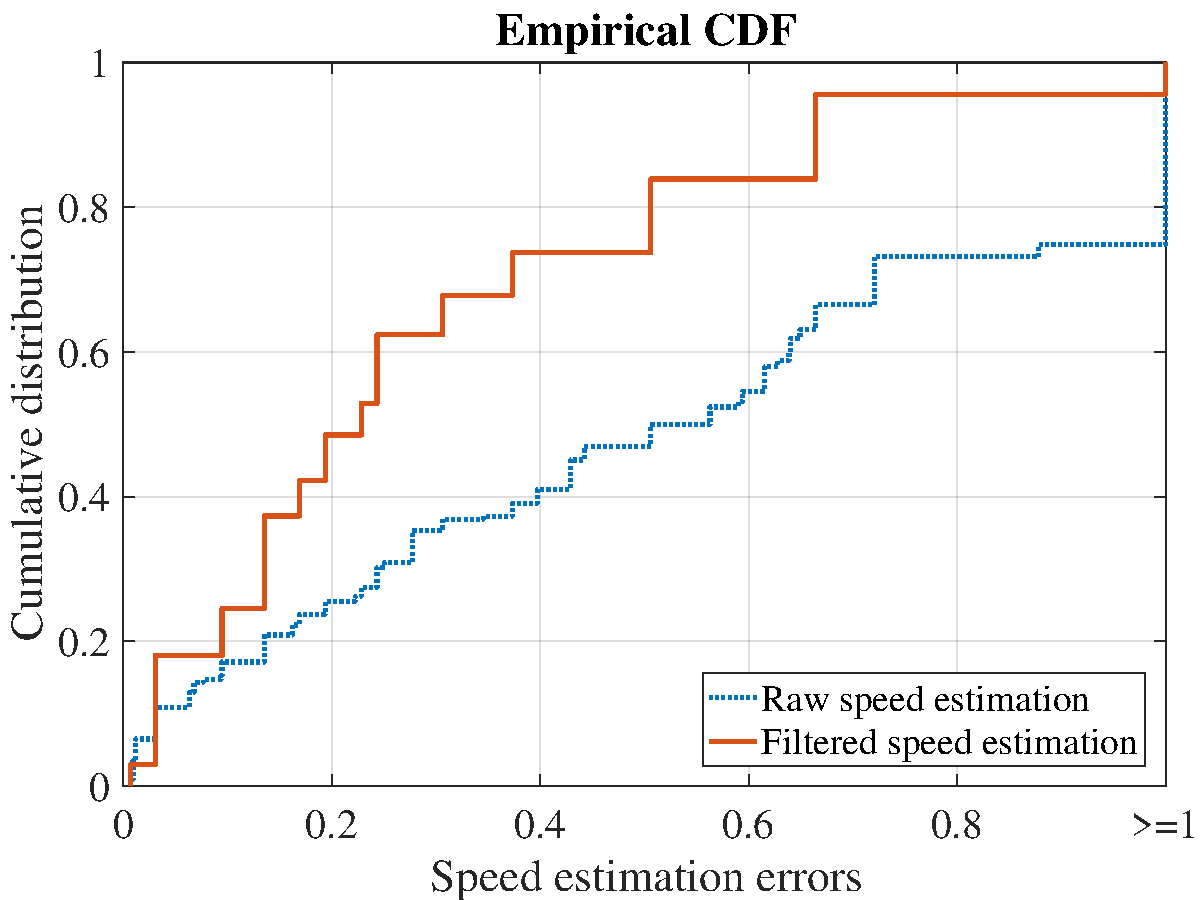
\includegraphics[width=0.5\linewidth]{./figures/cdf_limited.pdf}
    \caption{The CDF of raw speed estimation and filtered speed estimation}
    \label{fig:cdf_limited}
\end{figure}

As we can see in \autoref{fig:cdf_limited}, the filtered speed estimation significantly outperforms the raw speed estimation in terms of accuracy. About 50\% of the filtered speed estimates have error rates less than $0.2$, while only 25\% of raw speed estimates achieve the same level of accuracy. More than 80\% of filtered speed estimates have error rates less or equal to 0.5, while for raw speed estimates this number is only less than 50\%. On the other end of this figure, observe that there is only less than 5\% of filtered speed estimates with error rates higher than 1, compared to more than 15\% of raw speed estimates.


\begin{figure}[h]
    \centering
    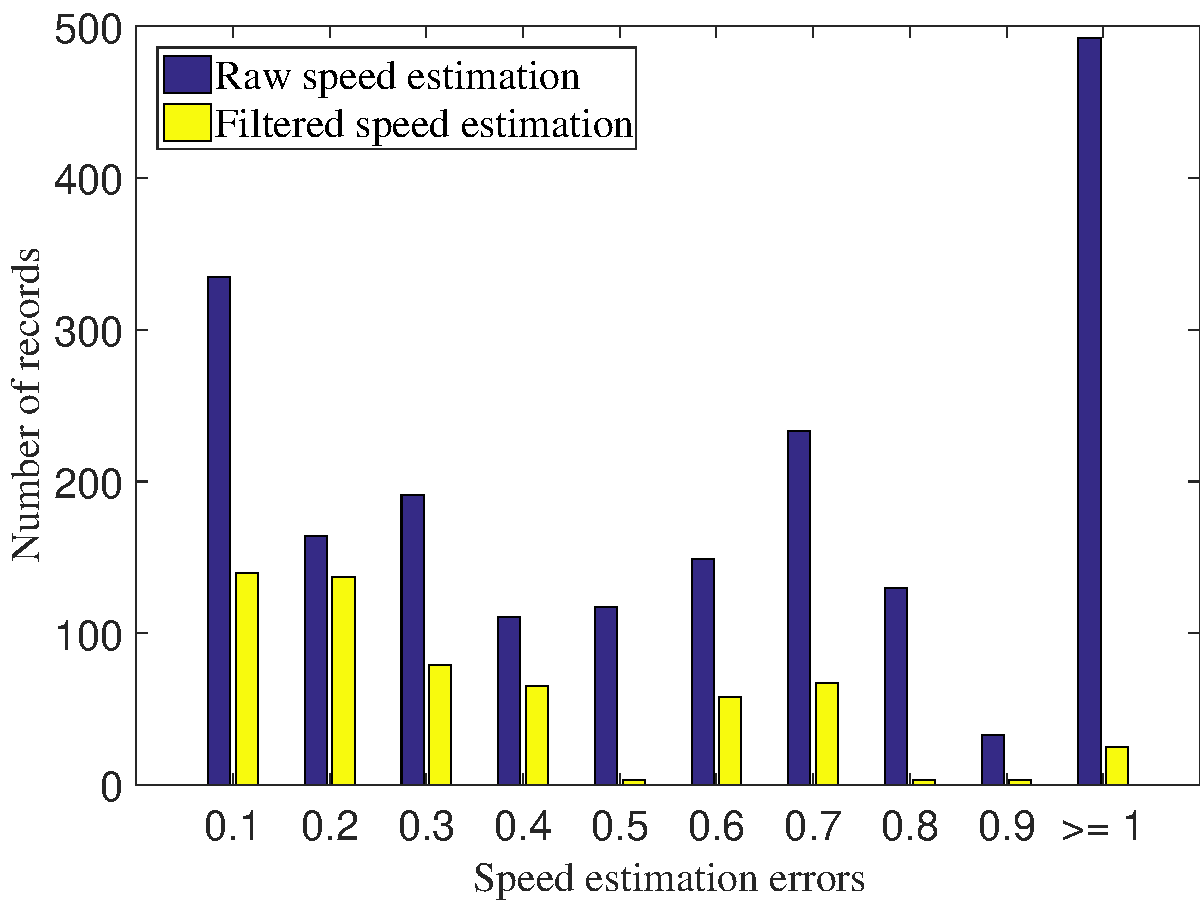
\includegraphics[width=0.5\linewidth]{./figures/error_bar.pdf}
    \caption{Number of records in each error bracket for raw speed estimation and filtered speed estimation}
    \label{fig:error_bar}
\end{figure}


\subsection{Speed Filtering}

\autoref{fig:error_bar} shows the number of records in each speed estimation error range, from 0.1 to 1 with an interval of 0.1. Observe that our speed estimation algorithm works well compared to raw estimates. For example, we can observe that approximately 50\% of records that have raw speed estimation errors less than 0.5 have been filtered out, while more than 85\% of records that have raw speed estimation errors greater than 0.5 have been filtered out.
